			\section{Figure e grafici}

Una relazione tecnico-scientifica raramente può essere considerata compiuta e dettagliata se priva di tabelle, figure e grafici grazie ai quali è possibile desumere anche empiricamente l'andamento delle misure e dei calcoli eseguiti.

Grafici, figure e tabelle non solo consentono di elaborare sotto altra forma l'informazione misurata o calcolata, ma permettono anche di estrapolare dati in modo implicito.

L'importanza dei grafici è anche confermata dai \textit{datasheet}%%
%%
\footnote{Il \textit{datasheet} non è altro che la documentazione tecnica di un particolare componente, dispositivo, eccetera.}
%%
dei componenti, degli strumenti et al, in cui vengono messe in risalto importanti caratteristiche elettriche, meccaniche o fisiche di altro tipo. Si osservi per esempio la figura~\ref{fig:datasheet} che riporta la pagina~17 di un datasheet dei \textit{supercapacitori} della {\sffamily\textit{muRata}}. Si noti l'uso dei grafici in cui viene messo in evidenza l'andamento della curva di scarica dei condensatori e tramite i quali è possibile dedurre rapidamente informazioni non esplicitamente fornite.

\begin{figure}[htb!]
\centering
    \includegraphics[width=0.7\textwidth]{figure/datasheet.pdf}%
    \caption{Particolare di un datasheet dei \textit{supercap} della {\sffamily\textit{muRata}}.}
    \label{fig:datasheet}
\end{figure}


				\subsection{Dare forma, corpo e anima ai dati: grafici}

Secondo studi americani di psicologia della comunicazione, delle cose lette, viste e ascoltate la mente umana conserva:
%%
\begin{itemize}
 \item il $10\%$ di ciò che legge;
 %%
 \item il $20\%$ di ciò che ascolta;
 %%
 \item il $30\%$ di ciò che vede;
 %%
 \item il $50\%$ di ciò che vede e ascolta.
\end{itemize}

L'importanza di un'illustrazione o di un grafico, si spiega quindi con la relativa facilità con cui la mente umana percepisce, elabora, assimila e interpreta linee e forme che strutturano l'informazione su piani diversi da quelli puramente numerici.

Ovviamente i grafici (figure, illustrazioni eccetera) con cui si vuole estendere il contenuto informativo di un documento, devono attenersi a criteri e requisiti che è doveroso rispettare.

Una delle regole, forse la più importante, è che ogni figura venga accompagnata da una breve didascalia che ne spieghi, brevemente, il significato. È anche buona norma, specie nei documenti più lunghi, far precedere la didascalia da un prefisso seguito da un numero come per esempio    ``\textbf{Fig.~<n>}'', ``\textbf{Figura~<n>}'' oppure, nel caso augurabile che il testo sia diviso in sezioni (raramente in capitoli), da prefissi e numerazioni come ``\textbf{Fig.~<m.n>}'' o ``\textbf{Figura~<m.n>}'' dove ``\textbf{n}'' indica il numero della figura e ``\textbf{m}'' il numero della sezione (o capitolo) in cui compare (si veda a proposito quanto adottato nelle figure e tabelle che accompagnano questo stesso documento).

Tale pratica diventa necessaria quando, nel corpo del testo, occorra far riferimento, anche più volte e in più pagine, a una specifica figura che compare in una determinata pagina. In tal caso ci si riferirà alla figura utilizzando formule come ``\textit{\ldots~ in fig.~2 a pag.~5 viene messo in evidenta~\ldots}'' o anche ``\textit{\ldots~la fig.~2 di pag.~5 spiega come~\ldots}''.

La didascalia va posta immediatamente sotto la figura o, anche se raramente e in alcuni stili tipografici, anche a lato.

Nel caso di immagini fotografiche o figure riconducibili a illustrazioni di natura non esattamente tecnico-scientifica, il formato grafico può essere \hlight{jpeg} (noto anche come \hlight{jpg}), o \hlight{png}. Si sconsiglia il formato \hlight{TIFF} per le notevoli dimensioni con cui l'immagine viene salvata e il formato \hlight{bmp}%%
%%
\footnote{\hlight{JPEG} è l'acronimo di \textsc{\hlight{J}oint \hlight{P}hotographic \hlight{E}xpert \hlight{G}roup} teso a definire uno standard per la compressione di immagini digitali. Il formato \hlight{PNG} è l'acronimo di \textsc{\hlight{P}ortable \hlight{N}etwork 
\hlight{G}raphics} che definisce un formato di file per la memorizzazione, la compressione e la gestione delle trasparenze di immagini. \hlight{TIFF} è l'acronimo di \textsc{\hlight{T}agged \hlight{I}mage \hlight{F}ile \hlight{F}ormat} e supporta immagini multiple, documenti multipagina possono quindi essere memorizzati in un unico file \hlight{tiff}. Il formato \hlight{BMP}, noto anche come Windows \textsc{Bitmap}, assegnando a ogni pixel un ben determinato valore cromatico, non consente la compressione dei file.}
%%
perché non offre le trasparenze e non possiede un algoritmo in grado di ottimizzare le dimensioni dei file al pari dei formati \hlight{jpg} e \hlight{png}. Da scartare infine le immagini di tipo \hlight{gif}, perché limitando a soli $8$~bit il numero dei colori, non garantisce immagini di buona qualità.

Se le immagini da inserire provengono da fonti fotografiche o ad esse riconducibili o illustrazioni, i formati \hlight{jpg} e \hlight{png} sono da preferire, perché il primo offre compressioni anche notevoli con relativa perdita di qualità, il secondo anche la possibilità di gestire le trasparenze.

Se per converso le immagini si riferiscono a schemi di qualsiasi tipo (elettrico, meccanico), a parti di apparecchiature, segni e simboli grafici, a meno di impedimenti o difficoltà particolari, improrogabili o ineliminabili, si raccomanda il salvataggio dell'immagine in uno dei tanti formati vettoriali che i programmi tecnici mettono sempre a disposizione (valutare anche la possibilità di ``\textit{stampare su file}'' tramite una cosiddetta \textit{stampante virtuale}).

I formati vettoriali più comuni sono:
%%
\begin{itemize}
 \item il \hlight{PDF}, acronimo di \textsc{\hlight{P}ortable \hlight{D}ocument \hlight{F}ormat};
 %%
 \item l'\hlight{SVG}, acronimo di \textsc{\hlight{S}calable \hlight{V}ector \hlight{G}raphics};
 %%
 \item il \hlight{DXF}, acronimo di \textsc{\hlight{D}rawing e\hlight{X}change \hlight{F}ormat};
 %%
 \item il \textsc{\hlight{P}ost\hlight{S}cript} o \hlight{PS};
 %%
 \item l'\textsc{\hlight{E}ncapsulated \hlight{P}ost\hlight{S}cript} o \hlight{EPS},
\end{itemize}
%%
e consentono di ridimensionare l'immagine senza alcuna perdita di qualità o dettaglio%%
%%
\footnote{Generalmente le immagini vettoriali non sono file binari, ma file di testo che contengono coordinate di punti che collegano tra loro semirette, cirve di \textit{Bezier}, \textit{spline} e altri tipi di curve parametriche.}.

Che si usi un'immagine di tipo \textit{raster} (le \hlight{jpg}, \hlight{png} \ecc) o una di tipo vettoriale, nel caso nasca l'esigenza di adattare l'immagine alle dimensioni del foglio o a una sua porzione, è importante che il ridimensionamento avvenga rispettando le proporzioni, possibilità offerta da praticamente tutti i software per l'elaborazione, conversione e trattamento di dati.


					\subsection{Rappresentazione dei dati: l'occhio vuole la sua parte}

Stabilito il formato grafico con cui memorizzare le immagini --preferibilmente vettoriale-- non resta altro che stabilire come rappresentare i dati disponibili.

\begin{figure}[htp!]
 \centering
 \subfloat[Grafico che mostra l'andamento di una sinusoide (per esempio quello di una corrente elettrica alternata).]{\label{subfig:sinusoide}%
	\includegraphics[width=0.44\textwidth]{figure/0_sinusoide.pdf}}
\qquad
 \subfloat[Grafico che mostra come in uno stesso sistema di assi cartesiani sia possibile \textit{costruire} più curve attribuibili ad altrettante funzioni.]{\label{subfig:sincos}%
	\includegraphics[width=0.44\textwidth]{figure/0_sincos.pdf}}
%\medskip

 \subfloat[Un grafico può anche mostrare come si distribuiscono i punti estrapolati per esempio da una serie di misure.]{\label{subfig:listplot}%
	\includegraphics[width=0.44\textwidth]{figure/0_listplot.pdf}}
\qquad
 \subfloat[Funzioni matematiche, grandezze fisiche, valori statistici \ecc possono essere rappresentate anche nello spazio.]{\label{subfig:plot3d}%
	\includegraphics[width=0.44\textwidth]{figure/0_plot3d.pdf}}
%\medskip

 \subfloat[Un grafico cosiddetto a \textit{istogramma} può essere utile per mostrare la differenza tra due o più dati.]{\label{subfig:barchart}%
	\includegraphics[width=0.44\textwidth]{figure/0_barchart.pdf}}
\qquad
 \subfloat[Un grafico a \textit{torta} mostra invece la distribuzione di due o più dati.]{\label{subfig:piechart}%
	\includegraphics[width=0.44\textwidth]{figure/0_piechart.pdf}}
%%%%
 \caption{Esempi di grafici}
 \label{fig:esempi_grafici}%\vspace{-1em}
\end{figure}

Si protrebbe infatti rappresentare l'andamento delle osservazioni approssimandole a quello di una funzione nota come nelle figure~\ref{subfig:sinusoide} e \ref{subfig:sincos} a pag.~\pageref{fig:esempi_grafici}. Misure e calcoli potrebbero anche essere rappresentati con una serie di linee e di punti come in figura~\ref{subfig:listplot} oppure, nel caso di misure che coinvolgono due variabili indipendenti, essere descritti nello spazio tridimensionale come in figura~\ref{subfig:plot3d}.

Le informazioni possono essere rappresentate anche in funzione della loro distribuzione. \hlight{Istogrammi} come quelli di figura~\ref{subfig:barchart} o \hlight{diagrammi a torta} come in figura~\ref{subfig:piechart}, potrebbero essere utilizzati, per esempio, per confrontare il valore di un certo numero di resistenze con medesimi \textit{dati di targa} costruite dal un'azienda in un certo periodo, con quelli di resistenze con gli stessi dati di targa e costruiti dalla medesima azienda ma in periodi differenti.

\begin{figure}[htpb]
	\centering
	\subfloat[Curve di fase e attenuazione di un filtro passa banda passivo. L'asse delle ascisse (frequenza) è in scala logaritmica.]{%
		\includegraphics[width=0.5\textwidth]{figure/graph_log.pdf}\label{subfig:filtro_log}%
	}
\hfill
	\subfloat[Stesso filtro e stesse curve caratteristiche della figura a sinistra. L'asse delle ascisse è in scala lineare.]{%
		\includegraphics[width=0.5\textwidth]{figure/graph_lin.pdf}\label{subfig:filtro_lin}%
	}
	\caption{Caratteristiche di fase e attenuazione di un filtro passa banda passivo su scala logaritmica e scala lineare.}
	\label{fig:filtro_pb}
\end{figure}

Un grafico si dice \hlightit{quantitativo} se sugli assi compaiono valori numerici dove sono anche indicate le unità di misura, si dice invece \hlightit{qualitativo} nel caso in cui vengano semplicemente indicati andamenti e tendenze (per esempio lo studio dell'andamento di una funzione matematica).

L'andamento di una grandezza, viene anche stabilito dalle caratteristiche attribuite agli assi cartesiani del piano (o dello spazio) su cui si intende rappresentarlo.

Come devono essere organizzati i dati? Su scala \textit{lineare} o \textit{logaritmica}? E la scala scelta vale per entrambi gli assi o su uno solo? L'ascissa o l'ordinata?

La scelta dipende ovviamente  dalla natura dei dati che devono essere rappresentati, dai loro valori minimi e massimi e da come \textit{fluttuano} le curve%%
%%
\footnote{Una curva potrebbe per esempio avere un particolare andamento in un range iniziale di valori piuttosto piccolo e un altro, però insignificante o non interessante, nel range di valori restante che però è molto esteso.}.
%%

Un modo con cui rappresentare dati e curve lungo un insieme esteso di valori consiste nell'usare, per uno o per entrambi gli assi, la \hlightit{scala logaritmica}.

\afterpage{\clearpage} %% serve per il flushing dell'immagine grande

Tale scala, proprio per le proprietà offerte dai logaritmi, permette di tracciare grandezze che pur estendendosi lungo uno degli assi --tipicamente quello delle ascisse-- per diversi ordini di grandezza, permette di mantenere un dettaglio relativo costante.

Le scale logaritmiche vengono anche usate per rappresentare unità di misura come il \hlightit{decibel} (dB), usato per misurare guadagni o attenuazioni di potenza e di tensione:
%%
\[
 A_p = 10\log\frac{P_u}{P_i}\,[\text{dBm}] \quad ; 
						\quad A_v = 20\log\frac{V_u}{V_i}\,[\text{dB}]
\]

Dove $P_u$, $V_u$, $P_i$ e $V_i$ sono rispettivamente potenza e tensione di uscita e potenzia e tensione di ingresso.

Siano per esempio i grafici di figura~\ref{fig:filtro_pb} relativi alla risposta in frequenza di un filtro \hlightit{passa-basso}. Il grafico di figura~\ref{subfig:filtro_log} utilizza per l'asse delle ascisse su cui è riportata la frequenza una scala logaritmica, mentre quello di figura~\ref{subfig:filtro_lin} una semplice scala lineare.

Si nota immediatamente che mentre il primo grafico a sinistra permette di apprezzare cosa accade alla fase e all'attenuazione alla frequenza di taglio del filtro ($-3\decibel$ a circa $160\Hz$) e nelle decadi successive (a $1600\Hz$, $16.000\Hz$ \ecc l'attenuazione aumenta ogni volta di $20\decibel$), quello a destra con ascissa lineare non consente di estrarre informazioni sufficientemente precise se non impossibili.


				\subsection{Costruzione di una scala logaritmica}

Si voglia rappresentare sull'asse delle ascisse un range piuttosto vasto di frequenze che, di decade in decade, vanno da $1\Hz$ fino a $1\MHz$. L'insieme delle frequenze è quindi:
%%
\[
 f:=\{1\Hz, 10\Hz, 100\Hz, 1\kHz, 10\kHz, 100\kHz, 1\MHz \}
\]

Per ognuna delle frequenze dell'insieme $f$, si devono calcolare i rispettivi logaritmi in base $10$:
%%
\begin{align*}
 &\log(1)=0 \quad\text{;}\quad \log(10)=1 \quad\text{;}\quad 
					\log(100)=\log(10^2)=2*\log(10)=2 \\
 &\log(1000)=\log(10^3)=3*\log(10)=3 \quad\text{;}\quad
					\log(10*10^3)=\log(10^4)=4*\log(10)=4 \\
 &\log(100*10^3)=\log(10^2*10^3)=\log(10^5)=5*\log(10)=5 \\
 &\log(10^6)=6*\log(10)=6
\end{align*}

Sull'asse delle ascisse si prende poi come riferimento un'unità di misura \hlight{$u$} ($2\cm$, $4\cm$ o il valore che si ritiene più opportuno) e si pone come origine dell'asse il valore corrispondente al $\log(1)$ (ovvero $0$) come in figura~\ref{fig:howtolog}\maroon{a}.
%%
\begin{figure}[ht!p]
\centering
    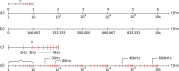
\includegraphics[width=\textwidth]{figure/scala_log_1.pdf}%
    \caption{Costruzione di una scala logaritmica}
    \label{fig:howtolog}
\end{figure}

Prendendo come riferimento l'unità di misura \hlight{$u$} stabilita, si segnano sulla parte superiore dell'ascissa i valori che vanno da $0$ a $6$ e, in corrispondenza di ognuno di essi, gli argomenti dei logaritmi che li hanno \textit{generati}, ovvero le frequenze che vanno da $1\Hz$ a $1\MHz$.

Per confronto si osservi invece l'ascissa di figura~\ref{fig:howtolog}\maroon{b} ricavata dividendo semplicemente in sei parti uguali il limite superiore del range di frequenza. In corrispondenza dei $10\Hz$ della scala logaritmica si hanno $166.667\Hz$ su quella lineare, in corrispondenza dei $1000\Hz$ di quella logaritmica si arriva a ben $500.000\Hz$ (cinquecentomila) su quella lineare.

I valori più bassi di frequenza della scala logaritmica subiscono, fino a poco più di metà range, un'espansione che poi man mano si comprime permettendo così di leggere cosa accade proprio in quelle frazioni di frequenza iniziali.

Naturalmente anche le porzioni intermedie di frequenza dovranno essere tracciate su scala logaritmica. Si prenda allora come riferimento la porzione di frequenza della 
figura~\ref{fig:howtolog}\maroon{a} che va da $1\Hz$ a $10\Hz$ che si è stabilito essere pari all'unità di misura \hlight{$u$} e che corrisponda per esempio a $25\mm$.

Al logaritmo di $1\Hz$ corrisponde come già detto il valore $0$, mentre al logaritmo di $10\Hz$ corrisponde il valore $1$.

Ciò che occorre fare, è calcolare i valori dei logaritmi intermedi che vanno da $2\Hz$ a $9\Hz$ che, moltiplicati per l'unità di misura \hlight{$u=25\mm$}, forniranno la distanza delle tacche dall'origine:
%%
\begin{align*}
 p_1 &= \log(2)*25 = 7,5\mm & p_2 &= \log(3)*25 = 11,9\mm & p_3 &= \log(4)*25 = 15,1\mm \\
 %%
 p_4 &= \log(5)*25 = 17,5\mm & p_5 &= \log(6)*25 = 19,5\mm & p_6 &= \log(7)*25 = 21,1\mm \\
 %%
 p_7 &= \log(8)*25 = 22,6\mm & p_8 &= \log(9)*25 = 23,9\mm & &
\end{align*}
%%
dove $p_1, p_2, \ldots, p_8$ sono le distanze delle singole tacche dall'origine. Si ottiene quindi la suddivisione mostrata in figura~\ref{fig:howtolog}\maroon{c} (scalata il doppio per mettere in evidenza la suddivisione) che, riportata intervallo dopo intervallo sull'asse delle ascisse di figura~\ref{fig:howtolog}\maroon{a}, suddivide infine l'ascissa logaritmica come in figura~\ref{fig:howtolog}\maroon{a}.

I diagrammi logaritmici dove uno degli assi è graduato linearmente sono detti \hlightit{semilogaritmici} (abbreviate anche come \hlightit{lin-log}); quelli in cui uno degli assi è invece espressione di valori calcolati con funzioni logaritmiche, sono invece detti \hlightit{bilogaritmici} (\hlightit{log-log}, vedi figura~\ref{subfig:filtro_log} dove l'ordinata destra è l'attenuazione espressa in $\decibel$).


					\subsection{Caratteristiche di un grafico}

Molto spesso, specie per la misura di grandezze fisiche affette da errori sistematici, è utile rappresentare non solo le curve o le spezzate definite da dati calcolati o dalle misure eseguite, ma anche gli errori ad esse correlate come in figura~\ref{fig:errori}
%%
\begin{figure}[ht!pb]
\centering
    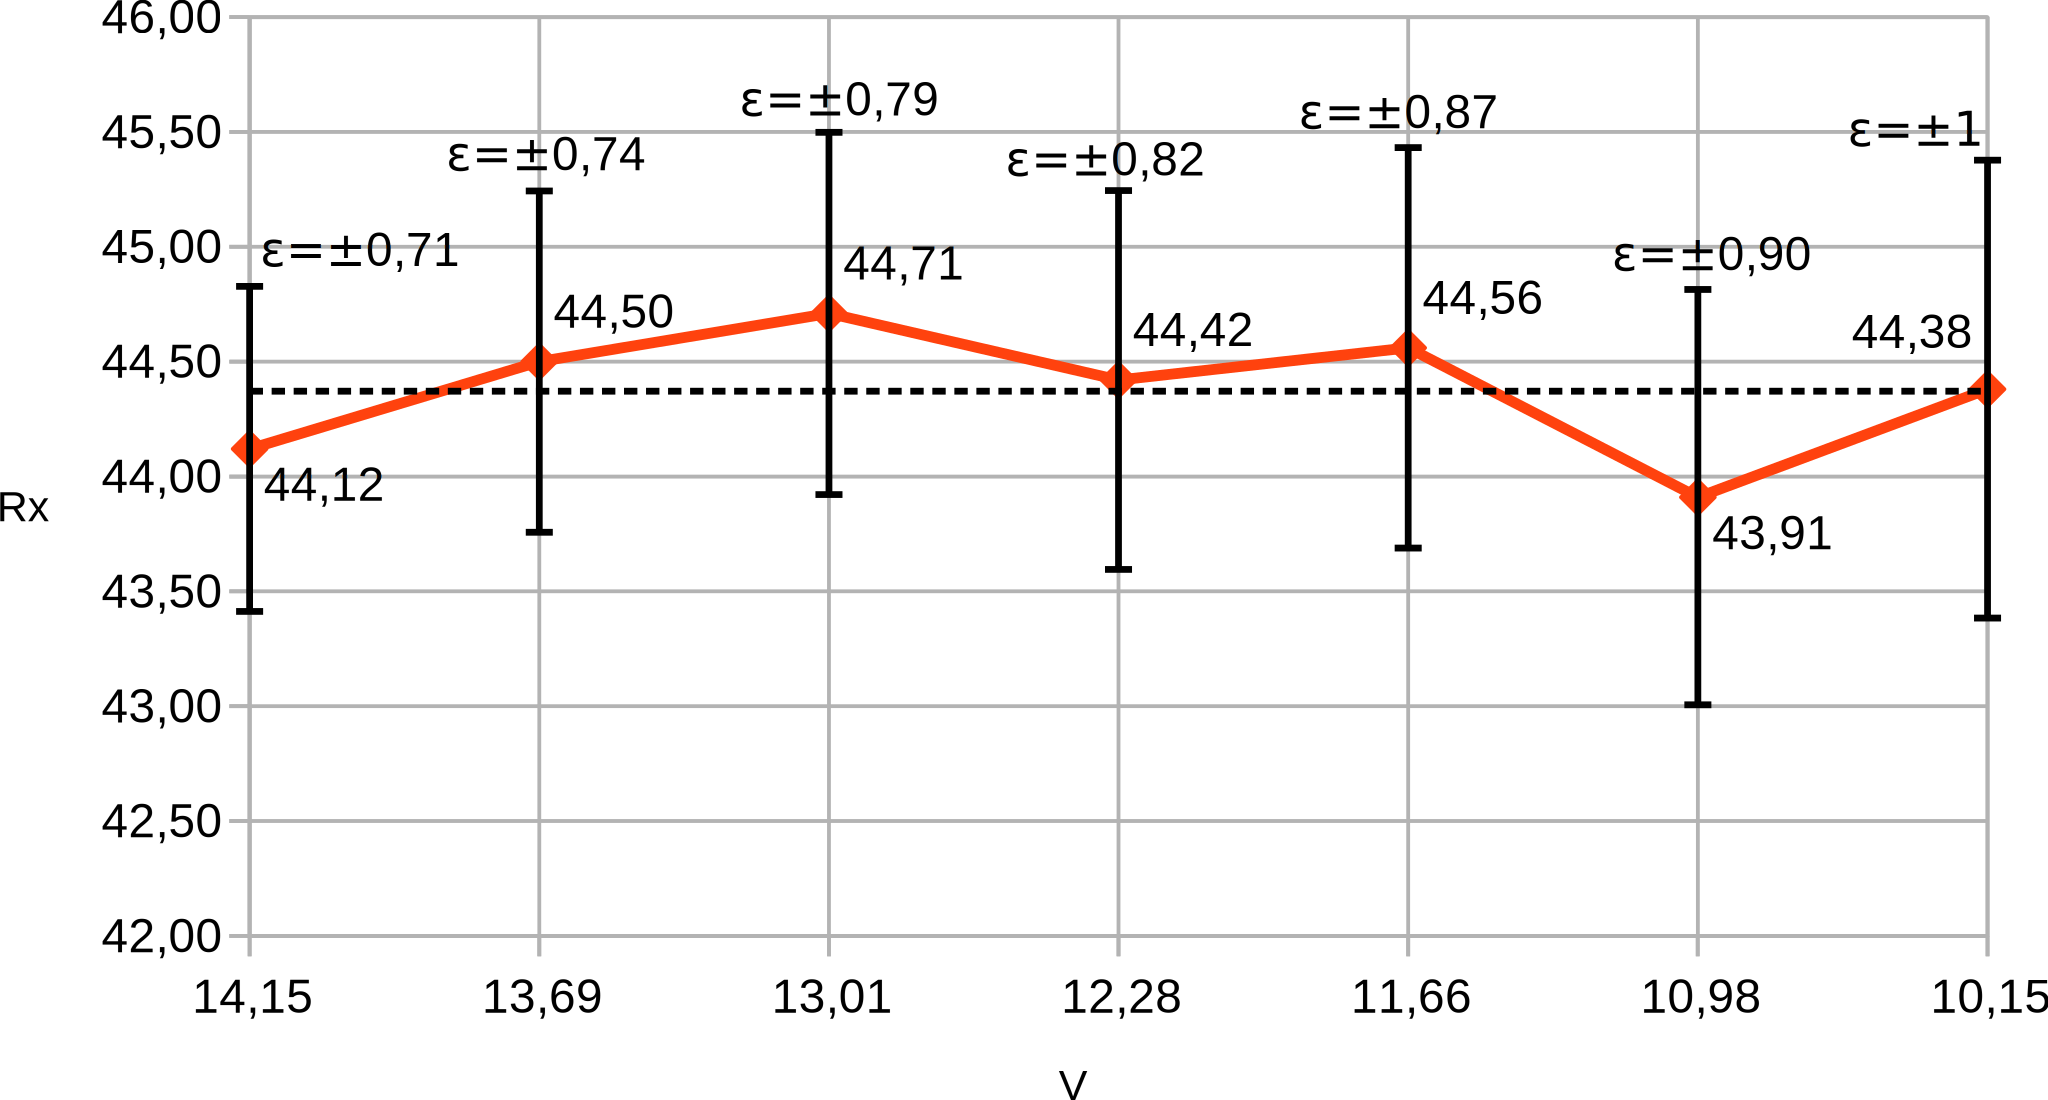
\includegraphics[width=0.8\linewidth]{figure/resistenza_con_errore.pdf}%
    \caption{Caratteristica di una curva in cui sono messi in evidenza gli errori $\eass$.}
    \label{fig:errori}
\end{figure}
%%
dove punto per punto, misura per misura, sono messe in evidenza le \textit{incertezze} (linee verticali).

Non di rado può essere utile rappresentare gli andamenti dei valori massimi e minimi delle misure in modo da mettere in evidenza il \textit{tunnel} entro cui si muove il valore centrale.

Le linee verticali vengono dette \hlightit{barre di errore} e indicano un intervallo di \textit{confidenza} o \textit{incertezza} (ovvero l'errore) relativo alle misure.

Il modo con cui i dati vengono visualizzati non è questione da poco, 
%%
\begin{figure}[htp]
	\centering
	\subfloat[Spezzate che uniscono i punti delle misure.]{%
		\includegraphics[width=0.5\textwidth]{figure/grafico_resistenza.pdf}\label{subfig:caratt_graph_a}%
	}
\hfill
	\subfloat[Linee descritte tramite interpolazione lineare.]{%
		\includegraphics[width=0.5\textwidth]{figure/interpolazione_polinomiale_resistenza.pdf}\label{subfig:caratt_graph_b}%
	}
	\caption[Caratteristiche delle linee di un grafico.]{Caratteristiche delle linee di un grafico: tramite spezzate o tramite interpolazione lineare.}
	\label{fig:caratt_graph}
\end{figure}

Per esempio, i punti della figura~\ref{subfig:caratt_graph_a} sono uniti tra loro da spezzate che, insieme, danno luogo all'\hlightit{interpolazione lineare}. Tale costruzione grafica non permette però di determinare in maniera efficace e men che meno precisa (al netto dell'errore comunque esistente) cosa accade nei punti intermedi.

Altro modo di rappresentare lo stesso insieme di tati è quello di ricorrere all'\hlightit{interpolazione polinomiale} in modo da descrivere, tramite curve e se possibile, il probabile valore di punti che non appartengono all'insieme dei dati misurati (figura~\ref{subfig:caratt_graph_b}).



					\section{Il luogo dei dati: le tabelle}

Una tabella è uno schema organizzato per righe e per colonne in cui inserire informazioni secondo un determinato criterio.

Le tabelle, quando unite a una efficacie rappresentazione grafica, sono uno degli strumenti più potenti con cui mostrare e riassumere gruppi correlati di dati.

Le informazioni provenienti da misure prese sul campo o elaborate attraverso analisi successive, possono essere così numerose che il loro uso nel testo o in formule ripetitive, possono determinare più confusione che chiarezza.

Raccogliere quindi tali informazioni in strumenti come tabelle, rende più facile e meno \textit{ingombrante} la lettura del testo.

Non va infatti dimenticato che una relazione, specie se tecnico-scientifica, deve godere di otto proprietà:
%%
\begin{enumerate}
 \item autorevolezza sulla modalità con cui vengono raccolti i dati e loro qualità;
 %%
 \item descrizione tecnicamente e grammaticamente inconfutabile;
 %%
 \item uso di un numero di pagine strettamente necessario;
 %%
 \item uso di adeguate teorie e formulazione di appropriate ipotesi;
 %%
 \item uso di adatti metodi per la misura del o dei fenomeni che si stanno osservando;
 %%
 \item uso appropriato di formule e grafici;
 %%
 \item analisi dei dati e verifica delle ipotesi;
 %%
 \item deduzioni e conclusioni.
\end{enumerate}

Un tabella diventa efficace se ben progettata e se possiede una struttura che consenta di leggere facilmente le singole informazioni. Una delle difficoltà maggiori consiste nel saper riconosce i dati che vanno organizzati per righe e per colonne e se, eventualmente, non sia il caso di dividerli in più tabelle.

Una tabella deve essere sempre identificata da una descrizione --la \hlightit{didascalia}-- che, al contrario delle figure, va posta sempre in alto. Come giù detto per le figure, la didascalia è bene che venga preceduta da un prefisso e da un numero consecutivo, con cui poterla identificare e richiamare in altre parti del testo (per esempio \maroon{Tab.\,1}, \maroon{Tabella\,1}, \maroon{Tab.1.2}, \ecc).


				\subsection{Struttura di una tabella}

Come accennato una tabella non è altro che una matrice formata da righe e colonne. In corrispondenza di ogni intersezione riga-colonna, detta \hlight{cella}, viene posto il dato.

La struttura più classica e completa di una tabella è quella di figura~\ref{fig:tab_index}
%%
\begin{figure}[htp!b!]
\centering\small
    \tabindice
    \caption{Parti di una tabella.}
    \label{fig:tab_index}
\end{figure}
%%
dove si riconosce una \hlightit{colonna indice} e un elenco di voci dette \hlightit{entrate} che indicizzano le colonne successive appartenenti a una stessa riga. Un banale esempio di colonna indice è la tabella~\ref{tab:tabindex} dove la prima colonna indica il numero della prova a cui i valori presenti nelle colonne seguenti si riferiscono.
%%
\begin{table}[h!tp]
 \centering\small
 \caption{Esempio di una tabella con colonna indice.}
 \tabesempioaA
 \label{tab:tabindex}
\end{table}

L'indicizzazione diventa utile nei casi in cui occorra riferirsi a uno o più valori ottenuti nel corso di una determinata misura.

Quando si progetta una tabella, le prime righe in alto sono sempre occupate dalle \hlightit{intestazioni} che specificano la natura della colonna e quindi dei dati posti nelle righe seguenti%%
%%
			\footnote{Nella tabella~\ref{tab:tabindex}, le intestazioni specificano che i valori presenti nelle righe che seguono sono letture di tensione, corrente o quelli della resistenza calcolata.}.
%%
Le intestazioni come quelle della tabella~\ref{tab:tabindex}, \textit{Voltometro} e \textit{Amperometro}, possono anche estendersi su più di una colonna quando, le informazioni contenute su più di una colonna, interessano un comune strumento, una comune grandezza, un comune fenomeno o altro ancora.

Nel caso in cui l'intestazione definisca grandezze fisiche, occorre anche specificare l'unità di misura, facendo eventualmente ricorso a opportuni multipli o sottomultipli, a cui i valori delle righe che seguono si riferiscono. In questo modo si evita non solo di dover ripetere per ogni valore l'unità di misura, ma anche l'inutile ripetizione di una informazione che appesentirebbe, specie nelle tabelle strutturalmente più complesse, la lettura.

Nel caso in cui il dato di una determinata cella non sia disponibile, al suo posto vengono inseriti tre punti o tre trattini.


					\subsection{Filetti, linee e griglie di una tabella: orrori da evitare}

Molti sono pronti a credere che una tabella sia effettivamente tale, solo se righe e colonne vengono delimitate da \hlightit{filetti} (\textit{linee}) verticali e orizzontali come nella tabella~\ref{tab:grigliata}.
%%
\begin{table}[htp]
 \centering\small
 \caption{Tabella con griglia. Errore da evitare.}
 \tabgrigliata
 \label{tab:grigliata}
\end{table}

Tabelle simili, specie se composte da un numero non indifferente di righe e colonne, sono assolutamente da evitare perché affaticano la vista e rendono le tabelle stesse meno leggibili.

Si crede infatti che il miglior modo per separare un dato da un altro, sia il tratto di linea che delimita e confina le informazioni contenute nelle singole celle.

L'alternativa esiste ed è quella paradossalmente ritenuta meno plausibile: usare pochissimi tratti di linea. Si confronti la grafica della tabella~\ref{tab:tabindex} a pagina~\pageref{tab:tabindex}, con quella della tabella con griglie. Leggera e più leggibile la prima, pesante e soffocante l'altra.

Con tre sole linee orizzontali si è dato alla tabella un aspetto graficamente e tipograficamnete migliore: due linee delimitano in alto e in basso la tabella, una terza linea, di spessore minore, separa invece le intestazioni dalle righe contenenti i dati.

Naturalmente il numero delle linee da utilizzare varia in base alla complessità della tabella. Come mostrato nella tabella~\ref{tab:tabindex}, altre due linee vengono utilizzate per delimitare, orizzontalmente, le intestazioni relative al \textit{Voltometro} e all'\textit{Amperometro}. La regola è: non esiste una regola se non quella di evitare assolutamente tabelle \textit{grigliate}.

Per dare il senso di alternanza delle righe di una tabella, si può utilizzare l'escamotage di colorare alternativamente le righe con un tenue punto di grigio in modo da migliorare, per così dire, la selettività visiva delle informazioni come in tabella~\ref{tab:alternata}.
%%
\begin{table}[htp]
 \centering\small
 \caption[Tabella con righe colorate alternativamente.]{Tabella con righe colorate alternativamente. Viene mantenuta la leggerezza grafica della tabella e contemporaneamente si è aumentata la distanza visiva tra una riga e un'altra senza l'uso di linee orizzontali.}
 \tabalternata
 \label{tab:alternata}
\end{table}

Si raccomanda, a meno di esigenze o richieste tipografiche particolari e tipiche comunque delle brochure o di documenti \textit{patinati}, l'uso di colori in tinta grigia chiara. Colori quali il rosso, il blu o anche il verde (ritenuto visivamente riposante, rischiano di affaticare la vista e di affogare le informazioni in inutili \textit{scale cromatiche}.

Una tabella  può naturalmente essere anche predisposta per raccogliere non solo informazioni di tipo numerico, ma anche informazioni prevalentemente testuali o grafiche (per esempio una tabella destinata a raccogliere la simbologia utilizzata in un particolare documento).

Un esempio è dato dalla tabella~\ref{tab:testuale} dove la colonna indice viene utilizzata per definire i periodi geologici. Trattandosi pur sempre di una tabella che per definizione assolve alla funzione di prospetto riassuntivo, la lunghezza del testo deve essere limitata a quella strettamente necessaria.
%%
\begin{table}[htp]
 \centering\small
 \caption[Tabella testuale.]{Tabella testuale. Si noti la possibilità di spezzare le linee di testo presenti in ciascuna cella.}
 \tabtestuale
 \label{tab:testuale}
\end{table}








